\section{Background}

X-rays are a type of ionizing electromagnetic radiation with typical energies in the \unit{\kilo\electronvolt} range. Their
production inside an X-ray tube relies on the electrostatic acceleration of electrons which then interact with the anode material. The main
mechanisms for the emission of energetic photons are the continuous bremsstrahlung resulting from electron deceleration as well as a
discrete component emitted after penetration of the inner atomic shells.



\subsection{Refractive index}

In classical ray optics, the laws of reflection and refraction according to Snell are
\begin{align*}
	\theta_i = \theta_r \: , && n_1 \cos\theta_i = n_2 \cos\theta_t \: ,
\end{align*}
where $n_1$ and $n_2$ are the refractive indices of the two media and $\theta_i, \theta_r, \theta_t$ are the angles of incidence, reflection
and transmission as shown in Figure \ref{fig:fresnel}.

\begin{figure}
	\centering
	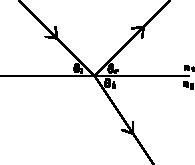
\includegraphics[width=0.33\textwidth]{content/graphics/fresnel.pdf}
	\caption{Depiction of reflection and refraction of light rays on a smooth surface.}
	\label{fig:fresnel}
\end{figure}

\begin{equation*}
	n = 1 - \delta + i\beta
\end{equation*}



\subsection{Fresnel coefficients}

Fresnel's formulae\footnote{Following the derivation in \cite{McMorrow_2011} among others.}

\subsection{Kiessig fringes}

\cite{Kiessig_1931}

\begin{figure}
	\centering
	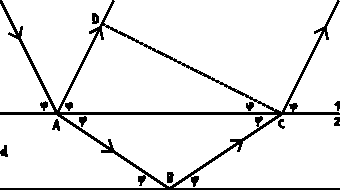
\includegraphics[width=0.55\textwidth]{content/graphics/kiessig.pdf}
	\caption{Schematic light paths inside a thin layer atop a substrate producing Kiessig oscillations according to \cite{Kiessig_1931}.}
	\label{fig:kiessig}
\end{figure}


\subsection{Stratified media}

\cite{Parratt_1954}

\begin{figure}
	\centering
	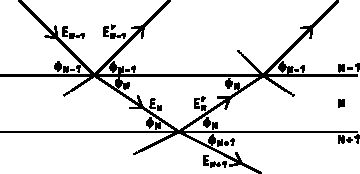
\includegraphics[width=0.66\textwidth]{content/graphics/parratt.pdf}
	\caption{Conceptual visualization of the Parratt algorithm presented in \cite{Parratt_1954}.}
	\label{fig:parratt}
\end{figure}

\cite{xray}
